\begin{frame}{Fonds Charcot\footnote{\url{https://patrimoine.sorbonne-universite.fr/collection/Fonds-Charcot}}}
	\begin{variableblock}{SorbonNum\\
			\footnotesize{Bibliothèque de Sorbonne Université (\textsc{BSU})}}{bg=white,fg=deepblue}{bg=blue,fg=pink}
		201 documents XML OCRisés (sans post-correction)
	\end{variableblock}
	%\begin{itemize}
	%    \item \textrm{Charcot} : textes rédigés par Charcot
	%    \item \textrm{Autres} : textes rédigés par les membres de son réseau scientifique
	%\end{itemize}
	\begin{table}[!ht]
		\centering
		\begin{tabular}{|c|r|r|}
			\hline 
			\rowcolor{yellow!30}
			Corpus & \multicolumn{1}{c|}{Nb de docs} & \multicolumn{1}{c|}{Nb de tokens} \\
			\hline
			\begin{tabular}[c]{@{}c@{}}\textrm{Charcot}\\ \scriptsize{textes rédigés par Charcot}\end{tabular}  & 68 & 12 190 649 (38,12\%) \\
			\hline
			\begin{tabular}[c]{@{}c@{}}\textrm{Autres}\\ \scriptsize{textes rédigés par les membres} \vspace{-0.15cm} \\ \scriptsize{de son réseau scientifique}\end{tabular}    & 133 & 19 788 830 (61,88\%) \\
			\hline\hline
			\textbf{Total} & \textbf{201} & \textbf{31 979 479} (100\%)\\
			\hline
		\end{tabular}
		\caption{Répartition du fonds Charcot selon les auteurs.
			%    \footnote{\tiny{\url{https://patrimoine.sorbonne-universite.fr/collection/Fonds-Charcot}}}
		}
		\label{tab:my_label}
	\end{table}
\end{frame}

\begin{frame}{Formalisation de l'approche}
	Extraction des concepts $\rightarrow$ problème d’extraction de la terminologie
	\begin{figure}[!h]
		\centering
		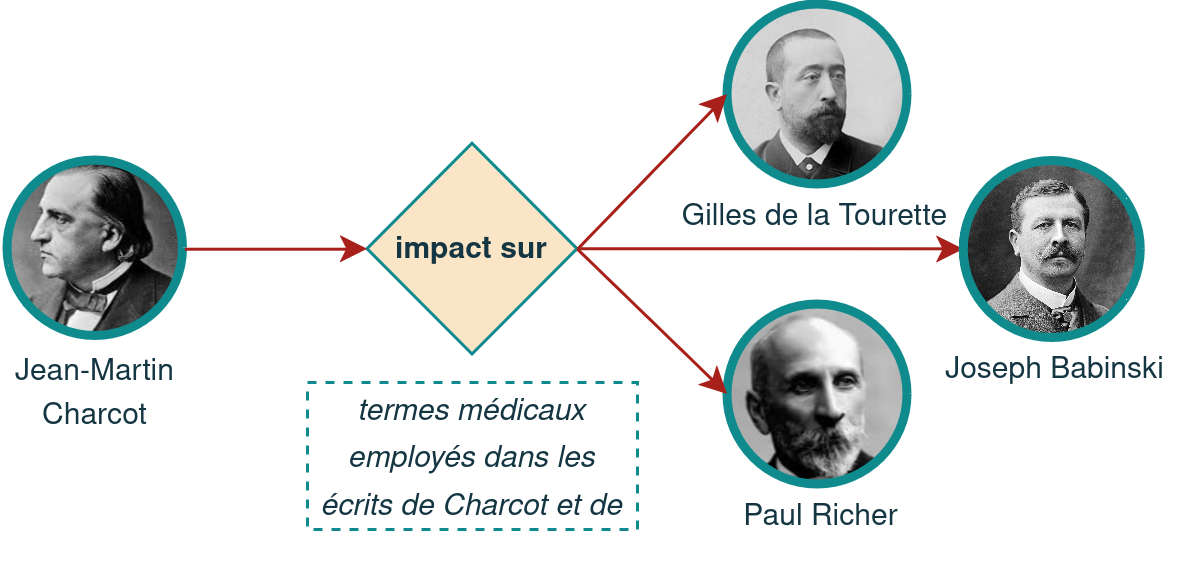
\includegraphics[width=100mm,scale=0.5]{pic/charcot_intertextualite.png}
		\caption{Opérationnalisation de l'impact de Charcot sur ses élèves.}
		\label{fig:my_label}
	\end{figure}
\end{frame}


\begin{frame}{Liste des concepts médicaux -- vérité terrain}
	Extraction semi-automatique des termes en lien avec Charcot.\\{\scriptsize\url{https://github.com/ljpetkovic/Charcot\_circulations/tree/main/concepts}}
	
	\begin{figure}[!htb]
		\centering
		\begin{minipage}{.5\textwidth}
			\centering
			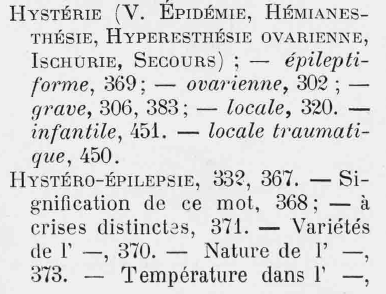
\includegraphics[width=0.6\linewidth, height=0.3\textheight]{pic/concepts-pdf}
			\caption{Index des termes \citep{charcot1892oeuvres}.}
			\label{fig:prob1_6_2}
		\end{minipage}%
		\begin{minipage}{.5\textwidth}
			\centering
			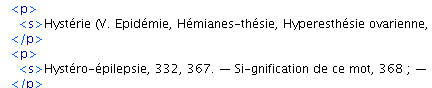
\includegraphics[width=1\linewidth, height=0.15\textheight]{pic/concepts-xml}
			\caption{Concepts médicaux, document XML.}
			\label{fig:prob1_6_1}
		\end{minipage}
	\end{figure}
 \begin{figure}[!htb]
	\centering
	\begin{minipage}{.5\textwidth}
		\centering
		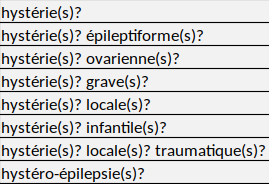
\includegraphics[width=0.6\linewidth, height=0.25\textheight]{pic/concepts-csv}
		\caption{Liste finale des concepts médicaux.}
		\label{fig:prob1_6_2}
	\end{minipage}%
	\begin{minipage}{.6\textwidth}
		\centering
		\begin{enumerate}
			\setcounter{enumi}{0}
			\item entre \texttt{<s>} et \texttt{,-(} (regex)
			\item sans termes génériques (\textit{os}, \textit{peau})
			\item prise en compte des sg. / pl. (regex)
		\end{enumerate}
	\end{minipage}
\end{figure}
\end{frame}

